\documentclass[11pt]{report}
\usepackage[a4paper]{geometry}
\usepackage{outline}
\usepackage{pmgraph}
\usepackage[normalem]{ulem}
\usepackage{graphicx}
\usepackage{booktabs}
\usepackage{amsmath}
\usepackage{amsthm}
\usepackage{eucal}
\usepackage{amssymb}
\usepackage{mathrsfs}
\usepackage{tikz}
\usepackage{pgf}
\usetikzlibrary{arrows,automata}
\usepackage{verbatim}
\usepackage{float}
\usepackage{appendix}
\allowdisplaybreaks
\usepackage{tkz-berge}
\usepackage{listings}
\usepackage{multirow}
\usepackage{color}
\lstset{language=matlab,frame=single}
\usepackage[framed,numbered,autolinebreaks,useliterate]{mcode}
\setcounter{secnumdepth}{5}
\setcounter{tocdepth}{4}



\title{\textbf{PageRank and Random Walks on the Web}}
\author{Shannon Chatha}
\date{\today}
%--------------------Make usable space all of page
\setlength{\oddsidemargin}{0in}
\setlength{\evensidemargin}{0in}
\setlength{\topmargin}{0in}
\setlength{\headsep}{-.25in}
\setlength{\textwidth}{6.5in}
\setlength{\textheight}{8.5in}
%--------------------Indention
\setlength{\parindent}{1cm}

\begin{document}


%--------------------Title Page
\maketitle
\begin{abstract}
This project...
\end{abstract}
\newpage
\vspace*{\fill}
\begin{center}
\textbf{Declaration of Authorship}\\ 
\textit{This piece of work is a result of my own work except where it forms an assessment
based on group project work. In the case of a group project, the work
has been prepared in collaboration with other members of the group. Material
from the work of others not involved in the project has been acknowledged and
quotations and paraphrases suitably indicated.}
\end{center}
\vspace*{\fill}

\newpage
\tableofcontents
%\addcontentsline{toc}{chapter}{Contents}
\listoffigures
\begingroup
\let\clearpage\relax
\listoftables
\endgroup
\addcontentsline{toc}{chapter}{List of Figures}
\addcontentsline{toc}{chapter}{List of Tables}
%--------------------Introduction

\chapter{Introduction}
Google's PageRank algorithm, developed in 1998 by Sergey Brin and Larry Page is one of the most well-known and influential methods of ranking web pages. The hyperlink structure of the web is represented by a directed graph, with the web pages representing the nodes and the links between nodes being the hyperlinks. Inlinks are pages that point into nodes, and outlinks point out from nodes \cite{brin1998anatomy}. The algorithm in its simplest form aims to rank pages with the assumption that a web page's importance is reliant on other important pages linking to it. When this is represented mathematically, it becomes clear that the importance scores of the web pages relate to the stationary points of a Markov chain, and hence Markov theory and matrices can be used to solve the PageRank equation:
\begin{equation}
\boldsymbol{\pi} = \boldsymbol{\pi} \cdot \textbf{G}
\end{equation}
where \textbf{G} is the 'Google Matrix' and $\boldsymbol{\pi}$ is the set of ranked web pages \cite{langville}. We are able to interpret a web pages PageRank as the fraction of time that a random surfer spends on that web page, with the random surfer more likely to return to the most important pages \cite{bonato}. Throughout this report we will be using the network graph as an example: 
\begin{figure}[H]
\centering
\begin{tikzpicture}[->,>=stealth',shorten >=1pt,auto,node distance=2cm,
                    semithick]
\tikzstyle{every state}=[fill=white,draw=black,text=black]
\node[state] (1) {$1$};
\node[state] (2) [right of=1] {$2$};
\node[state] (3) [right of=2] {$3$};
\node[state] (4) [below of=1] {$4$};
\node[state] (5) [below of=3] {$5$};
\node[state] (6) [below of=4] {$6$};
\node[state] (7) [right of=6] {$7$};
\node[state] (8) [right of=7] {$8$};
\path (1) edge node{} (2)
          edge node{} (4)
          edge [bend right] node{} (6)
      (2) edge node{} (3)
          edge node{} (5)
      (3) edge node{} (5)
      (4) edge node{} (7)
          edge node{} (5)
      (5) edge [bend right] node{} (8)
      (6) edge node{} (4)
          edge node{} (7)
          edge [bend right] node{} (8)
      (8) edge [bend right] node{} (5)
          edge node{} (7);
          
\end{tikzpicture}
\caption{Graph modelling 8-node web} \label{Example}
\end{figure}

In the first chapter of this report, we will explore mathematical representations of the PageRank equation, the modifications required on the matrix in order to use Markov theory to solve the PageRank equation, and finally on the use of the power method to solve the equation. Chapter 3 will then explore improvements to the PageRank representation that could increase the accuracy and personalise the PageRank method for a user, such as weighted PageRank and topic-specific PageRank. Chapter 4 discusses other methods of ranking web pages, and compares these to PageRank. Chapter 5 explores potential applications for PageRank beyond ranking web-pages, for example in predicting traffic flow in Durham. The final chapter of the report, Chapter 6, summarises the main points of the report.



%--------------------Matrix Representation 
\chapter{Mathematical Representation}
In this chapter we aim to represent the PageRank equation mathematically, in section 2.1, we use summation formulas to represent the algorithm, and introduce the idea of an iterative process to compute the PageRank vector. In section 2.2 we represent the PageRank equation using matrices, and discuss the two adjustments required in order to use Markov theory to solve the PageRank equation leading to the formation of a dense Google Matrix. We will discuss the use of the power method to solve the PageRank equation in section 2.3.

The references Austin \cite{austin}, Bonato \cite{bonato} and Langville \cite{langville} were consulted during the writing of this chapter, and the material has been collated below.  

\section{Summation Formula of PageRank}
In order to mathematically represent the PageRank algorithm, Brin and Page first assigned each page, $P_i$, a rank
\begin{equation}
r(P_i) = \displaystyle \sum_{P_j\in B_{P_i }} \frac{r(P_j)}{|P_j|}
\end{equation} where $B_{P_i}$ is the set of pages pointing into $P_i$, and $\vert P_j\vert$ is the number of outlinks from a page. However the ranking of outlinks is unknown, and so an iterative summation formula is required, where it is assumed that all pages have equal PageRank at the start, \(r_o = \frac{1}{n}\) , \begin{equation} \label{iterative}
r_{(k+1)}P_i = \displaystyle \sum_{P_j\in B_{P_i }}\frac{r_k(P_j)}{|P_j|}
\end{equation} When \eqref{iterative} is applied to all pages in the graph, you can calculate a ranking for the pages, so for the graph in figure \ref{Example}, we get the following values for the PageRanks after some iterations: 

 \begin{table}[H] \caption{First iterates using \eqref{iterative} on Figure \ref{Example}}
 \centering
 \begin{tabular} {c c c |c} 
 Iter. 0 & Iter. 1 & Iter. 2 &  Rank at Iter. 2 \\ [0.5ex] 
 \hline
 $r_0(P_1)=\frac{1}{8}$ & $r_1(P_1)=0$ & $r_2(P_1)=0$ & $6$ \\ 
 $r_0(P_2)=\frac{1}{8}$ & $r_1(P_2)=\frac{1}{24}$ & $r_2(P_2)=0$ & $6$ \\ 
 $r_0(P_3)=\frac{1}{8}$ & $r_1(P_3)=\frac{1}{16}$ & $r_2(P_3)=\frac{1}{48}$ & $4$ \\ 
 $r_0(P_4)=\frac{1}{8}$ & $r_1(P_4)=\frac{5}{48}$ & $r_2(P_4)=\frac{1}{48}$ & $4$ \\ 
 $r_0(P_5)=\frac{1}{8}$ & $r_1(P_5)=\frac{5}{16}$ & $r_2(P_5)=\frac{11}{48}$ & $2$ \\ 
 $r_0(P_6)=\frac{1}{8}$ & $r_1(P_6)=\frac{1}{24}$ & $r_2(P_6)=0$ & $6$ \\ 
 $r_0(P_7)=\frac{1}{8}$ & $r_1(P_7)=\frac{3}{16}$ & $r_2(P_7)=\frac{1}{6}$ & $3$ \\ 
 $r_0(P_8)=\frac{1}{8}$ & $r_1(P_8)=\frac{3}{16}$ & $r_2(P_8)=\frac{1}{3}$ & $1$ \\ \end{tabular}
\label{table1}
\end{table}

\section{Matrix Representation}
\subsection{Hyperlink Matrix}
If we represent the PageRank algorithm using matrices, we are able to compute a 1 x \textit{n} row vector, $\boldsymbol{\pi}^T$, the PageRank vector, at each iteration which contains the PageRank values for all web pages in the hyperlink graph. In order to do this we first introduce the concept of the Hyperlink matrix, a [\textit{n}x\textit{n}] matrix \textbf{H}, which is a row normalized matrix where 
\(\boldsymbol{H_{ij}} = \begin{cases} \frac{1}{\vert P_j \vert} & P_j\in B_{P_i } \\ 0 & \textnormal{otherwise} \end{cases}\). So for Figure \ref{Example} we are able to produce 
\[\textbf{H}=\left(
\begin{array}{cccccccc}
0 & \frac{1}{3} & 0 & \frac{1}{3} & 0 &\frac{1}{3} & 0& 0 \\
0 & 0 &\frac{1}{2}& 0 &\frac{1}{2}& 0 & 0 & 0\\
0 & 0 & 0 & 0 & 1 & 0 & 0 & 0\\
0 & 0 & 0 & 0 & \frac{1}{2} & 0 & \frac{1}{2} & 0\\
0 & 0 & 0 & 0 & 0 & 0 & 0 & 1\\
0 & 0 & 0 & \frac{1}{3} & 0 & 0 & \frac{1}{3} & \frac{1}{3} \\
0 & 0 & 0 & 0 & 0 & 0 & 0 & 0\\
0 & 0 & 0 & 0 & \frac{1}{2} & 0 & \frac{1}{2} & 0\\
\end{array}
\right)	\]

The non-zero elements of row \textit{i} relate to the outlinking pages of $P_i$, for example, node 1 has outlinks to pages 2, 4 and 6, and so in columns 2, 4 and 6 of \textbf{H} the value in row 1 are $\frac{1}{3}$ and the non-zero elements of column \textit{i} relates to the inlinking pages.

We are able to write \eqref{iterative} as \begin{equation}
\boldsymbol\pi^{(k+1)T} = \boldsymbol\pi^{(k)T}\textbf{H}
\end{equation} which shows that the vector $\boldsymbol\pi^T$ is an eigenvector of the matrix \textbf{H} with eigenvalue 1, otherwise known as the stationary vector of \textbf{H}, essentially this is the classical power method applied to \textbf{H}. We are able to observe that \textbf{H} is a very sparse matrix, as the majority of its entries are 0, which is computationally very beneficial, as it reduces the vector-matrix multiplication at each iteration to a linear computation. The formation of \textbf{H} is very similar to the formation of a transition probability matrix for a Markov chain, and it is also noted that \textbf{H} is similar to a stochastic matrix, as all entries are non-negative, however not all rows sum to 1.

From Markov theory, we know that for any starting vector, the power method applied to a matrix, \textbf{M},  will converge to a stationary vector as long as \textbf{M} is stochastic, irreducible and aperiodic. However, \textbf{H} is not guaranteed to converge due to the presence of rank sinks. A rank sink is a page that stores PageRank with each iteration, this can be in the form of dangling nodes, which are nodes that have no outlinks, for example 
\begin{figure}[h]
\centering
\begin{tikzpicture}[->,>=stealth',shorten >=1pt,auto,node distance=2cm,
                    semithick]
\tikzstyle{every state}=[fill=white,draw=black,text=black]
\node[state] (1) {$1$};
\node[state] (2) [right of=1] {$2$};
\node[state] (3) [right of=2] {$3$};
\path (1) edge node{} (2)
          edge [bend right] node{} (3)
      (3) edge [bend right] node{} (1)
          edge node{} (2);
\end{tikzpicture} \caption{Simple graph with rank sink} \label{dangling} 
\end{figure} in Figure \ref{dangling}, node 2 is a dangling node. There can also be an issue with cycles,
\begin{figure}[h]
\centering
\begin{tikzpicture}[->,>=stealth',shorten >=1pt,auto,node distance=2cm,
                    semithick]
\tikzstyle{every state}=[fill=white,draw=black,text=black]
\node[state] (1) {$1$};
\node[state] (2) [right of=1] {$2$};
\path (1) edge [bend right] node{} (2)
      (2) edge [bend right] node{} (1);
\end{tikzpicture} \caption{Simple graph with cycle} \label{cycle}
\end{figure} for example in Figure \ref{cycle}, an infinite loop is created between nodes 1 and 2, and so the iterate will not converge. We are able to apply modifications to \textbf{H} which make it a Markov matrix.

\subsection{Stochastic Matrix}
The first modification, called the stochasticity adjustment, leads to the formation of a stochastic matrix, \textbf{S}. In the stochasticity adjustment, we change rows of 0's to rows of $\frac{1}{n}$, hence making \textbf{S} stochastic, as all rows now sum to 1. Mathematically this is shown as, \begin{equation} \label{s}
\textbf{S} = \textbf{H} + \textbf{a}\left(\frac{1}{n}\cdot 1^{T}\right)
\end{equation} where \textbf{a} is the dangling node vector, \(\boldsymbol{a} = \begin{cases} 1 & \textnormal{if dangling node} \\ 0 & \textnormal{otherwise} \end{cases}\), and $1^T$ is the rank 1 matrix with unit entries of size [1x\textit{n}].

In terms of the random surfer idea as mentioned in section 1.1, this means that if the surfer enters a dangling node, it is able to teleport to another page in the graph at random. For the 8-node graph example in Figure \ref{Example}, we produce  
\[\textbf{S}=\left(
\begin{array}{cccccccc}
0 & \frac{1}{3} & 0 & \frac{1}{3} & 0 &\frac{1}{3} & 0& 0 \\
0 & 0 &\frac{1}{2}& 0 &\frac{1}{2}& 0 & 0 & 0\\
0 & 0 & 0 & 0 & 1 & 0 & 0 & 0\\
0 & 0 & 0 & 0 & \frac{1}{2} & 0 & \frac{1}{2} & 0\\
0 & 0 & 0 & 0 & 0 & 0 & 0 & 1\\
0 & 0 & 0 & \frac{1}{3} & 0 & 0 & \frac{1}{3} & \frac{1}{3} \\
\frac{1}{8} & \frac{1}{8} & \frac{1}{8} & \frac{1}{8} & \frac{1}{8} & \frac{1}{8} & \frac{1}{8} & \frac{1}{8}\\
0 & 0 & 0 & 0 & \frac{1}{2} & 0 & \frac{1}{2} & 0\\
\end{array}
\right)	\] This modification ensures that \textbf{S} is stochastic, but not that it is irreducible and aperiodic and so it is not guaranteed that it will converge when using the power method.

The stochasticity adjustment is especially crucial when modelling the web in practice, as in an analysis of a significant section of the web graph, only a quarter of the web is strongly connected, and so a large majority of the web are dangling nodes \cite{chakrabarti2002mining}.

\subsection{Google Matrix}
The primitivity adjustment is the next modification to the matrix which ensures that it is both aperiodic and irreducible. This modification introduces a scaling parameter $\alpha \in [0,1]$. In terms of the random surfer, this adjustment means that most of the time the surfer will follow links from page $P_i$ to $P_j$, however at any time the surfer could choose a page uniformly at random from the graph and jump there. This adjustment is shown by \begin{equation}\label{G}
\textbf{G}=\alpha\textbf{S}+\left((1-\alpha)\cdot\frac{1}{n}\cdot1^T\right)
\end{equation} where \textbf{G} is the Google matrix. For Figure \ref{Example},
\[\textbf{G}=\alpha\textbf{S}+\left((1-\alpha)\cdot \frac{1}{8} \cdot \left(  \begin{array}{cccccccc}
1&1&1&1&1&1&1&1\end{array}\right) \right)\]

Due to the primitivity adjustment, \textbf{G} is stochastic, as it is the combination of two stochastic matrices, irreducible and aperiodic. This implies that the power method applied to \textbf{G} is guaranteed to converge to a stationary vector $\boldsymbol{\pi}^T$. \begin{equation}\label{power to G}
\boldsymbol{\pi}^{(k+1)T} = \boldsymbol{\pi}^{(k)T}\textbf{G}
\end{equation} However, \textbf{G} is artificial, as it has been modified twice in order to assure convergence, also \textbf{G} is dense, which is a computational disadvantage, this can be solved by expressing \textbf{G} in terms of \textbf{H}, a very sparse matrix; 

 
\begin{align}
\textbf{G} & = \alpha\textbf{S}+\left((1-\alpha)\cdot\frac{1}{n}\cdot1^T\right)\notag\\
& = \alpha \left(\textbf{H} + \textbf{a}\left(\frac{1}{n}\cdot 1^{T}\right)\right) + \left((1-\alpha)\cdot\frac{1}{n}\cdot1^T\right)\notag\\
& = \alpha\textbf{H} + (\alpha\textbf{a} +(1-\alpha))\left(\frac{1}{n}\cdot 1^T\right)\label{G in H}
\end{align}

\subsection{$\alpha$ parameter}
The $\alpha$ parameter introduced in the primitivity adjustment controls how much the original hyperlink structure of the web is weighted. As $\alpha \rightarrow 1$ the expected number of iterations required before convergence increases as the PageRank vector is more volatile, however artificiality is low, and we are close to working with the original hyperlink graph. When $\alpha =0$ then $\textbf{G}=\frac{1}{n}\cdot 1^T$, so there is a link between every page, and so the hyperlink structure has completely disappeared. 

Brin and Page suggested the value of 0.85, as this strikes a balance between efficiency and effectiveness. Using Figure \ref{Example} and \eqref{G in H}, we obtain
\begin{equation}
\textbf{G} = \left(
\begin{array}{cccccccc}
0.019 & 0.302 & 0.019 & 0.302 & 0.019 & 0.302 & 0.019 & 0.019  \\
0.019 & 0.019 & 0.444 & 0.019 & 0.444 & 0.019 & 0.019 & 0.019  \\
0.019 & 0.019 & 0.019 & 0.019 & 0.869 & 0.019 & 0.019 & 0.019  \\
0.019 & 0.019 & 0.019 & 0.019 & 0.444 & 0.019 & 0.444 & 0.019  \\
0.019 & 0.019 & 0.019 & 0.019 & 0.019 & 0.019 & 0.019 & 0.869  \\
0.019 & 0.019 & 0.019 & 0.302 & 0.019 & 0.019 & 0.302 & 0.302  \\
0.125 & 0.125 & 0.125 & 0.125 & 0.125 & 0.125 & 0.125 & 0.125  \\
0.019 & 0.019 & 0.019 & 0.019 & 0.444 & 0.019 & 0.444 & 0.019 
\end{array}
\right)
\end{equation}
\section{Solving the PageRank Equation}
In order to solve the PageRank equation we either need to solve the eigenvector problem for $\boldsymbol{\pi}^T$, \(\boldsymbol{\pi}^T = \boldsymbol{\pi}^T\textbf{G}\), i.e. we need to find a normalized dominant left-hand eigenvector of \textbf{G} which corresponds to the dominant eigenvalue of $\lambda_1 = 1$. We are also able to solve the equation by using a linear system \(\boldsymbol{\pi}^T(\textbf{I}-\textbf{G})=\textbf{0}^T\), where we want to find a normalized left-hand vector of \textbf{I}-\textbf{G}, \cite{langville}. We will discuss the power method in more detail in this report, as this is the original method proposed to solve the PageRank equation \cite{langville}.


\cite{ipsen2005analysis}, \cite{page1999pagerank}
\subsection{Power Method}

\textcolor{red}{\textbf{EXPLAIN MATHS MORE HERE}}

Using matlab code as given in Appendix \ref{app:code}, 

\[\boldsymbol\pi = \left(
\begin{array}{c}
0.040 \\
0.051 \\
0.062 \\
0.066 \\
0.258 \\
0.051 \\
0.199 \\
0.274
\end{array}
\right)\]

\subsection{Why the Power Method}

The power method is useful for solving the PageRank equation as it converges to a unique vector, the PageRank vector, where the $i^{th}$ entry of $\boldsymbol\pi$ relates to the PageRank of \textit{i} \cite{ipsen2005analysis}. The main disadvantage of the power method is that it known to be very slow to converge, with the computation of the PageRank vector taking a few days to complete for the large web graph, but the power method is very simple. As we are able to simplify G to H as shown in \eqref{G in H}, the power method is very storage friendly, this is as for an iteration only a sparse \textbf{H}, a dangling node vector \textbf{a} and the current iterate are required to be stored \cite{langville}. Brin and Page reported that the PageRank vector converges to 2-3 degrees of accuracy within 50-100 iterations \cite{austin}.

%--------------------Improvements
\chapter{Improvements to the Algorithm}

In this chapter we will discuss various methods of improving the PageRank algorithm in order to improve the accuracy of the PageRank vector for a user. The original algorithm is simplistic in the assumption that a random surfer will move throughout the hyperlink graph without any bias, and so it is not very realistic, as a surfer will be more drawn to pages that interest them specifically, we will discuss this more with respect to the formulation of a Topic-specific PageRank algorithm. Another modified algorithm is the Weighted PageRank which takes into account the importance of the outlinks and inlinks a page has.

References: \cite{baeza2004web}, \cite{bonato}, , \cite{langville}, \cite{manning}, \cite{stata2000term}, \cite{thorson2004modeling}, \cite{tomlin2003new} 

\section{Weighted PageRank}\label{sec:weighted} \cite{xing2004weighted}

When weighted equations applied to example in Figure \ref{Example}, we produce a hyperlink matrix which is different to \textbf{H} produced in section 2.2.1 

\[\textbf{W}_{out}=\left(
\begin{array}{cccccccc}
0 & \frac{2}{7} & 0 & \frac{2}{7} & 0 &\frac{3}{7} & 0 & 0 \\
0 & 0 &\frac{1}{2}& 0 &\frac{1}{2}& 0 & 0 & 0\\
0 & 0 & 0 & 0 & 1 & 0 & 0 & 0\\
0 & 0 & 0 & 0 & 1 & 0 & 0 & 0\\
0 & 0 & 0 & 0 & 0 & 0 & 0 & 1\\
0 & 0 & 0 & \frac{1}{2} & 0 & 0 & 0 & \frac{1}{2} \\
0 & 0 & 0 & 0 & 0 & 0 & 0 & 0\\
0 & 0 & 0 & 0 & 1 & 0 & 0 & 0\\
\end{array}
\right)	\]

\[\textbf{W}_{in}=\left(
\begin{array}{cccccccc}
0 & 0 & 0 & 0 & 0 & 0 & 0 & 0 \\
0 & 0 & 0 & 0 & 0 & 0 & 0 & 0\\
0 & 1 & 0 & 0 & 0 & 0 & 0 & 0\\
0 & 0 & 0 & 0 & 0 & 1 & 0 & 0\\
0 & \frac{1}{6} & \frac{1}{6} & \frac{1}{3} & 0 & 0 & 0 & \frac{1}{3}\\
0 & 0 & 0 & 0 & 0 & 0 & 0 & 0 \\
0 & 0 & 0 & \frac{2}{5} & 0 & \frac{1}{5} & 0 & \frac{2}{5}\\
0 & 0 & 0 & 0 & \frac{4}{5} & \frac{1}{5} & 0 & 0\\
\end{array}
\right)	\]
\[\textbf{H}_{WPR}=\left(
\begin{array}{cccccccc}
0 & 0 & 0 & 0 & 0 & 0 & 0 & 0 \\
0 & 0 & 0 & 0 & 0 & 0 & 0 & 0\\
0 & 0 & \frac{1}{2} & 0 & \frac{1}{2} & 0 & 0 & 0\\
0 & 0 & 0 & \frac{1}{2} & 0 & 0 & 0 & \frac{1}{2}\\
0 & 0 & \frac{1}{12} & 0 & \frac{11}{12} & 0 & 0 & 0\\
0 & 0 & 0 & 0 & 0 & 0 & 0 & 0 \\
0 & 0 & 0 & \frac{1}{10} & \frac{8}{10} & 0 & 0 & \frac{1}{10}\\
0 & 0 & 0 & \frac{1}{10} & 0 & 0 & 0 & \frac{9}{10}\\
\end{array}
\right)	\]

Through the same methods as discussed in chapters 2 and 3, we produce a PageRank vector \[\boldsymbol\pi_{WPR} = \left(
\begin{array}{c}
0.028 \\
0.028 \\
0.097 \\
0.097 \\
0.395 \\
0.028 \\
0.028 \\
0.302
\end{array}
\right)\]
when we compare the PageRankings produced by performing the standard algorithm and the weighted algorithm:
\begin{table}[H] \caption{Comparison of PageRankings produced by standard algorithm and the weighted PageRank algorithm}
 \centering
 \begin{tabular} {c| c c} 
 Node & PR & WPR \\ [0.5ex] 
 \hline
 1&8&5\\
 2&6&5\\
 3&5&3\\
 4&4&3\\
 5&2&1\\
 6&6&5\\
 7&3&5\\
 8&1&2\\
 \end{tabular}
 \label{comparison}
\end{table}
\cite{langville}, \cite{xing2004weighted}, \cite{baeza2004web}
\section{Intelligent Surfer}
\cite{richardson2002intelligent}
\section{Personalization Vector}
\section{Topic Specific PageRank}
\cite{haveliwala1999efficient}, \cite{haveliwala2002topic}


%--------------------Comparison to other methods of Ranking webpages
\chapter{Other Methods of Ranking Web Pages}
References: \cite{baldi2003modeling}, \cite{bharat1998improved}, \cite{bonato}, \cite{ding2003pagerank}, \cite{farahat2006authority}, \cite{kleinberg1999authoritative}, \cite{langville}, \cite{lempel2000stochastic}, \cite{manning}, \cite{ng2001link}, \cite{ng2001stable}

\section{HITS method}
\begin{equation}
\textbf{L}=\left(
\begin{array}{cccccccc}
0 & 1 & 0 & 1 & 0 & 1 & 0 & 0 \\
0 & 0 & 1 & 0 & 1 & 0 & 0 & 0 \\
0 & 0 & 0 & 0 & 1 & 0 & 0 & 0 \\
0 & 0 & 0 & 0 & 1 & 0 & 0 & 0 \\
0 & 0 & 0 & 0 & 0 & 0 & 0 & 1 \\
0 & 0 & 0 & 1 & 0 & 0 & 0 & 1 \\
0 & 0 & 0 & 0 & 0 & 0 & 0 & 0 \\
0 & 0 & 0 & 0 & 1 & 0 & 0 & 0 \\
\end{array}
\right)
\end{equation}
\begin{equation}
\textnormal{Authority matrix} = \textbf{L}^T\textbf{L}=\left(
\begin{array}{cccccccc}
0 & 0 & 0 & 0 & 0 & 0 & 0 & 0 \\
0 & 1 & 0 & 1 & 0 & 1 & 0 & 0 \\
0 & 0 & 1 & 0 & 1 & 0 & 0 & 0 \\
0 & 1 & 0 & 2 & 0 & 1 & 1 & 1 \\
0 & 0 & 1 & 0 & 4 & 0 & 2 & 0 \\
0 & 1 & 0 & 1 & 0 & 1 & 0 & 0 \\
0 & 0 & 0 & 1 & 2 & 0 & 3 & 1 \\
0 & 0 & 0 & 1 & 0 & 0 & 1 & 2 \\
\end{array}
\right)
\end{equation}
\begin{equation}
\textnormal{Hub matrix} = \textbf{LL}^T=\left(
\begin{array}{cccccccc}
3 & 0 & 0 & 0 & 0 & 1 & 0 & 0 \\
0 & 2 & 1 & 1 & 0 & 0 & 0 & 1 \\
0 & 1 & 1 & 1 & 0 & 0 & 0 & 1 \\
0 & 1 & 1 & 2 & 0 & 1 & 0 & 2 \\
0 & 0 & 0 & 0 & 1 & 1 & 0 & 0 \\
1 & 0 & 0 & 1 & 1 & 3 & 0 & 1 \\
0 & 0 & 0 & 0 & 0 & 0 & 0 & 0 \\
0 & 1 & 0 & 2 & 0 & 1 & 0 & 2 \\
\end{array}
\right)
\end{equation}
Using matlab code as given in Appendix \ref{app:code}, we are able to compute authority score \textbf{x}, and hub score, \textbf{y}, vectors;
\begin{eqnarray}
\textbf{x}^T = \left( \begin{array} {cccccccc}
0 & 0.030 & 0.069 & 0.118 & 0.343 &0.030 &0.305 &0.106
\end{array}\right) \\
\textbf{y}^T = \left( \begin{array} {cccccccc}
0.062 & 0.144 & 0.120 & 0.226 & 0.037 & 0.185 & 0 & 0.226
\end{array}\right)
\end{eqnarray}
\section{SALSA method}
\begin{figure}[H]
\centering
\begin{tikzpicture}
   \begin{scope}[rotate=90]
       \SetVertexNoLabel
       \grEmptyLadder[RA=2,RB=6]{8}   
       \AssignVertexLabel{a}{8h,7h,6h,5h,4h,3h,2h,1h}
       \AssignVertexLabel{b}{8a,7a,6a,5a,4a,3a,2a,1a}

   \end{scope} 
   \EdgeFromOneToSel{b}{a}{0}{1,3}
   \EdgeFromOneToSel{b}{a}{1}{0,1,4}
   \EdgeFromOneToSel{b}{a}{3}{0}
   \EdgeFromOneToSel{b}{a}{4}{1,3} 
   \EdgeFromOneToSel{b}{a}{5}{3}
   \EdgeFromOneToSel{b}{a}{6}{5,3}
   \EdgeFromOneToSel{b}{a}{7}{2,4,6} 
\end{tikzpicture}\caption{Bipartite graph of Figure \ref{Example} } \label{bipartite}
\end{figure}

\begin{equation}
\textbf{L}_r=\left(
\begin{array}{cccccccc}
0 & \frac{1}{3} & 0 & \frac{1}{3} & 0 & \frac{1}{3} & 0 & 0 \\
0 & 0 & \frac{1}{2} & 0 & \frac{1}{3} & 0 & 0 & 0 \\
0 & 0 & 0 & 0 & 1 & 0 & 0 & 0\\
0 & 0 & 0 & 0 & \frac{1}{2} & 0 & \frac{1}{2} & 0 \\
0 & 0 & 0 & 0 & 0 & 0 & 0 & 1 \\
0 & 0 & 0 & \frac{1}{3} & 0 & 0 & \frac{1}{3} & \frac{1}{3} \\
0 & 0 & 0 & 0 & 0 & 0 & 0 & 0 \\
0 & 0 & 0 & 0 & \frac{1}{2} & 0 & \frac{1}{2} & 0 \\
\end{array}
\right)
\end{equation} 

\begin{equation}
\textbf{L}_c^T=\left(
\begin{array}{cccccccc}
0 & 0 & 0 & 0 & 0 & 0 & 0 & 0 \\
1 & 0 & 0 & 0 & 0 & 0 & 0 & 0 \\
0 & 1 & 0 & 0 & 0 & 0 & 0 & 0 \\
\frac{1}{2} & 0 & 0 & 0 & 0 & \frac{1}{2} & 0 & 0 \\
0 & \frac{1}{4} & \frac{1}{4} & \frac{1}{4} & 0 & 0 & 0 & \frac{1}{4}\\
1 & 0 & 0 & 0 & 0 & 0 & 0 & 0 \\
0 & 0 & 0 & \frac{1}{3} & 0 & \frac{1}{3} & 0 & \frac{1}{3} \\
0 & 0 & 0 & 0 & \frac{1}{2} & \frac{1}{2} & 0 & 0 \\
\end{array}
\right)
\end{equation}

\begin{equation}
\textbf{L}_r\textbf{L}_c^T=\left(
\begin{array}{cccccccc}
\frac{5}{6} & 0 & 0 & 0 & 0 & \frac{1}{6} & 0 & 0 \\
0 & \frac{5}{8} & \frac{1}{8} & \frac{1}{8} & 0 & 0 & 0 & \frac{1}{8} \\
0 & \frac{1}{4} & \frac{1}{4} & \frac{1}{4} & 0 & 0 & 0 & \frac{1}{4} \\
0 & \frac{1}{8} & \frac{1}{8} & \frac{7}{24} & 0 & \frac{1}{6} & 0 & \frac{7}{24} \\
0 & 0 & 0 & 0 & \frac{1}{2} & \frac{1}{2} & 0 & 0\\
\frac{1}{6} & 0 & 0 & \frac{1}{9} & \frac{1}{6} & \frac{4}{9} & 0 & \frac{1}{9} \\
0 & 0 & 0 & 0 & 0 & 0 & 0 & 0 \\
0 & \frac{1}{8} & \frac{1}{8} & \frac{7}{24} & 0 & \frac{1}{6} & 0 & \frac{7}{24} \\
\end{array}
\right)
\end{equation}

\begin{equation}
\textbf{L}_c^T\textbf{L}_r=\left(
\begin{array}{cccccccc}
0 & 0 & 0 & 0 & 0 & 0 & 0 & 0 \\
0 & \frac{1}{3} & 0 & \frac{1}{3} & 0 & \frac{1}{3} & 0 & 0 \\
0 & 0 & \frac{1}{2} & 0 & \frac{1}{2} & 0 & 0 & 0 \\
0 & \frac{1}{6} & 0 & \frac{1}{3} & 0 & \frac{1}{6} & \frac{1}{6} & \frac{1}{6} \\
0 & 0 & \frac{1}{8} & 0 & \frac{5}{8} & 0 & \frac{1}{4} & 0 \\
0 & \frac{1}{3} & 0 & \frac{1}{3} & 0 & \frac{1}{3} & 0 & 0 \\
0 & 0 & 0 & \frac{1}{9} & \frac{1}{3} & 0 & \frac{4}{9} & \frac{1}{9} \\
0 & 0 & 0 & \frac{1}{6} & 0 & 0 & \frac{1}{6} & \frac{2}{3} \\
\end{array}
\right)
\end{equation}

\begin{equation}
\textnormal{Hub Matrix}=\left(
\begin{array}{ccccccc}
\frac{5}{6} & 0 & 0 & 0 & 0 & \frac{1}{6} & 0 \\
0 & \frac{5}{8} & \frac{1}{8} & \frac{1}{8} & 0 & 0 & \frac{1}{8} \\
0 & \frac{1}{4} & \frac{1}{4} & \frac{1}{4} & 0 & 0 & \frac{1}{4} \\
0 & \frac{1}{8} & \frac{1}{8} & \frac{7}{24} & 0 & \frac{1}{6} & \frac{7}{24} \\
0 & 0 & 0 & 0 & \frac{1}{2} & \frac{1}{2} & 0\\
\frac{1}{6} & 0 & 0 & \frac{1}{9} & \frac{1}{6} & \frac{4}{9} & \frac{1}{9} \\
0 & \frac{1}{8} & \frac{1}{8} & \frac{7}{24} & 0 & \frac{1}{6} & \frac{7}{24} \\
\end{array}
\right)
\end{equation}

\begin{equation}
\textnormal{Authority Matix}=\left(
\begin{array}{ccccccc}
\frac{1}{3} & 0 & \frac{1}{3} & 0 & \frac{1}{3} & 0 & 0 \\
0 & \frac{1}{2} & 0 & \frac{1}{2} & 0 & 0 & 0 \\
\frac{1}{6} & 0 & \frac{1}{3} & 0 & \frac{1}{6} & \frac{1}{6} & \frac{1}{6} \\
0 & \frac{1}{8} & 0 & \frac{5}{8} & 0 & \frac{1}{4} & 0 \\
\frac{1}{3} & 0 & \frac{1}{3} & 0 & \frac{1}{3} & 0 & 0 \\
0 & 0 & \frac{1}{9} & \frac{1}{3} & 0 & \frac{4}{9} & \frac{1}{9} \\
0 & 0 & \frac{1}{6} & 0 & 0 & \frac{1}{6} & \frac{2}{3} \\
\end{array}
\right)
\end{equation}
Local Hub and Authority scores:


Global Hub and Authority scores:
\begin{eqnarray}
\pi_h = \left( \begin{array} {cccccccc}
0.188 & 0.125 & 0.063 & 0.125 & 0.063 & 0.188 & 0.125 & 0.125
\end{array}\right) \\
\pi_a = \left( \begin{array} {cccccccc}
0.125 & 0.063 & 0.063 & 0.125 & 0.250 & 0.063 & 0.188 & 0.125
\end{array}\right)
\end{eqnarray}

\section{Comparing PageRank, HITS and SALSA}

\begin{table}[H] \caption{Page rankings for Figure \ref{Example} using PR, HITS and SALSA }
 \centering
 \begin{tabular} {c| c| c| c| c| c} 
 \multirow{2}{*}{Node} & \multirow{2}{*}{PR} & \multicolumn{2}{|c|}{HITS} & \multicolumn{2}{|c}{SALSA} \\ [0.5ex] 
 {}&{}&Authority & Hub & Authority & Hub\\ 
 \hline
 1&8&1&3&8&6\\
 2&6&3&6&6&4\\
 3&5&7&6&5&5\\
 4&4&3&3&3&1\\
 5&2&7&1&1&7\\
 6&6&1&6&6&3\\
 7&3&3&2&2&8\\
 8&1&3&3&4&1\\
 \end{tabular}
 \label{comparison}
\end{table}

  
  
%--------------------Applications
\chapter{Applications of the PageRank algorithm}

The PageRank algorithm can also be used in many varied applications beyond ranking web pages \cite{gleich2015pagerank}, which we explore in this chapter. We will explore the algorithm with respect to modelling traffic in Durham in more detail, alongside applications in chemistry and in recommender systems. 

The PageRank algorithm can be used as a measure of network centrality, where you are able to understand a graph better when PageRank reveals what is most important. We are also able to apply modified PageRank to some applications, for example reverse PageRank can be used to model food chains, where a species,\textit{i}, is important if it feeds a species, \textit{j} \cite{allesina2009googling}. 

\section{Wikipedia}
We are able to apply PageRank to large databases such as Wikipedia, for example, we can generate reading lists for university courses automatically from exploiting the link structure of Wikipedia \cite{wissner2006preparation}. We are able to rank articles to find the top 100 historical figures and which cultures have the largest reach, for example a culture will have a high PageRank if it has many inlinks from other cultures. PageRank reveals that Carl Linnaeus is the most 'important' page due to the fact that he developed the scientific classification system we use for animals, insects and plants, and so these pages link back to him \cite{eom2015interactions}. We are also able to conclude that the most important figures in history are Western men who are born after the 17th Century. This mathematical analysis of historical figures and cultures using Wikipedia can be very useful in exploring interactions between world cultures and understanding history.


\section{Chemistry}
The PageRank algorithm has been used when studying molecules in chemistry, specifically in MoleculaRnetworks \cite{JCC:JCC22917}, which is a toolkit for identifying a shape of a solvent and exploring the H-bonding in that solvent. 
\begin{figure}
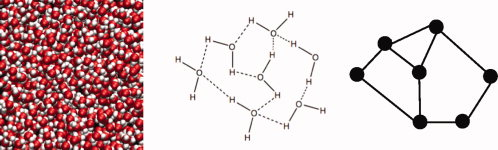
\includegraphics[width=\linewidth]{Decomposition_of_simulation_date_into_a_graph_-chem.jpg}
\caption{Decomposition of simulation data into a graph, \cite{JCC:JCC22917}}
\label{fig:chem}
\end{figure}
We are able to assess changes to the Hydrogen bond network due to the solute through the analysis of the network structure, as a graph is formed where the nodes are water molecules, and links represent potential hydrogen bonds, as shown in Figure \ref{fig:chem}. PageRank of each water molecule is determined by the number of edges connected to it, along with the number of edges connected to the nodes neighbours. As each polyhedron has its own unique PageRank vector, we are able to access a database in order to confirm the polyhedra structure. The use of PageRank is a novel way to extract chemical information, and can enhance the traditional methods used in chemical spectroscopy.

%\section{Recommender Systems}

%References:\cite{gori2007itemrank}
\section{Roads and Urban Networks}
We are able to apply the PageRank algorithm to road networks in order to predict traffic flow and also human movement. Jiang et al. found that weighted PageRank is the best metric with regards to correlating or predicting traffic flow \cite{1742-5468-2008-07-P07008}. A city can be topologically represented by a connectivity graph as shown in Figure \ref{city rep}, and as over 60\% of human movement can be predicted or explained using a connectivity graph \cite{doi:10.1080/13658810802022822}.

\begin{figure}[h]
\centering
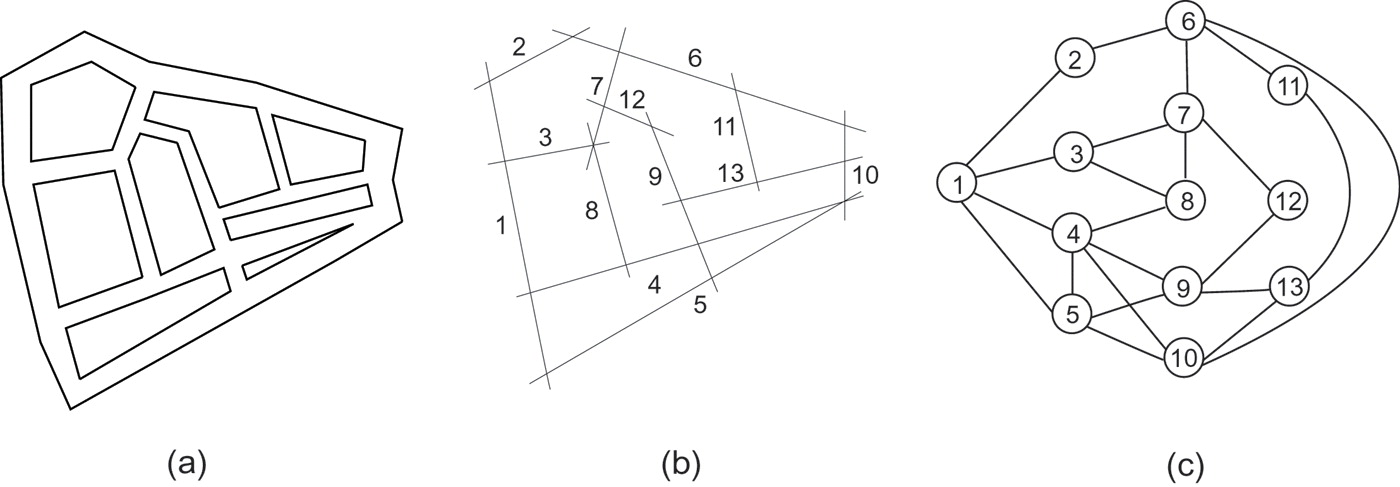
\includegraphics[width=\linewidth]{map_view.jpeg}
\caption{(a) A fictive urban system, (b) its axial map and (c) connectivity graph, taken from \cite{doi:10.1080/13658810802022822}}
\label{city rep}
\end{figure}

This application is slightly different to the usual PageRank algorithm, as the graph formed from a urban space is a connected graph, and so there are no dangling nodes involved, in terms of a random walker, they will never get stuck, we assume that they never get tired and that they always move to one of its successors with non-uniform probability, as well-connected streets are preferable. Due to this non-uniform probability, we need to use the weighted PageRank algorithm as discussed in Section \ref{sec:weighted} as opposed to the standard algorithm.



\subsection{Durham}
Jiang showed that PageRank scores are significantly correlated to human movement in four areas of London \cite{doi:10.1080/13658810802022822}, and we will use this methodology as a basis for our analysis of vehicle movement in Durham. 
\subsubsection{Methodology}
In order to represent the road network in Durham, we first produce an axial map and then are able to form a connectivity graph. The axial map is produced by taking a map of Durham, Figure \ref{durham map}, and representing the intersections of the roads by a 'The axial map is constructed by taking an accurate map and drawing a set of intersecting lines through all the spaces of the urban grid so that the grid is covered and all rings of circulation are completed.'\cite{space}



\begin{figure}[h]
\centering
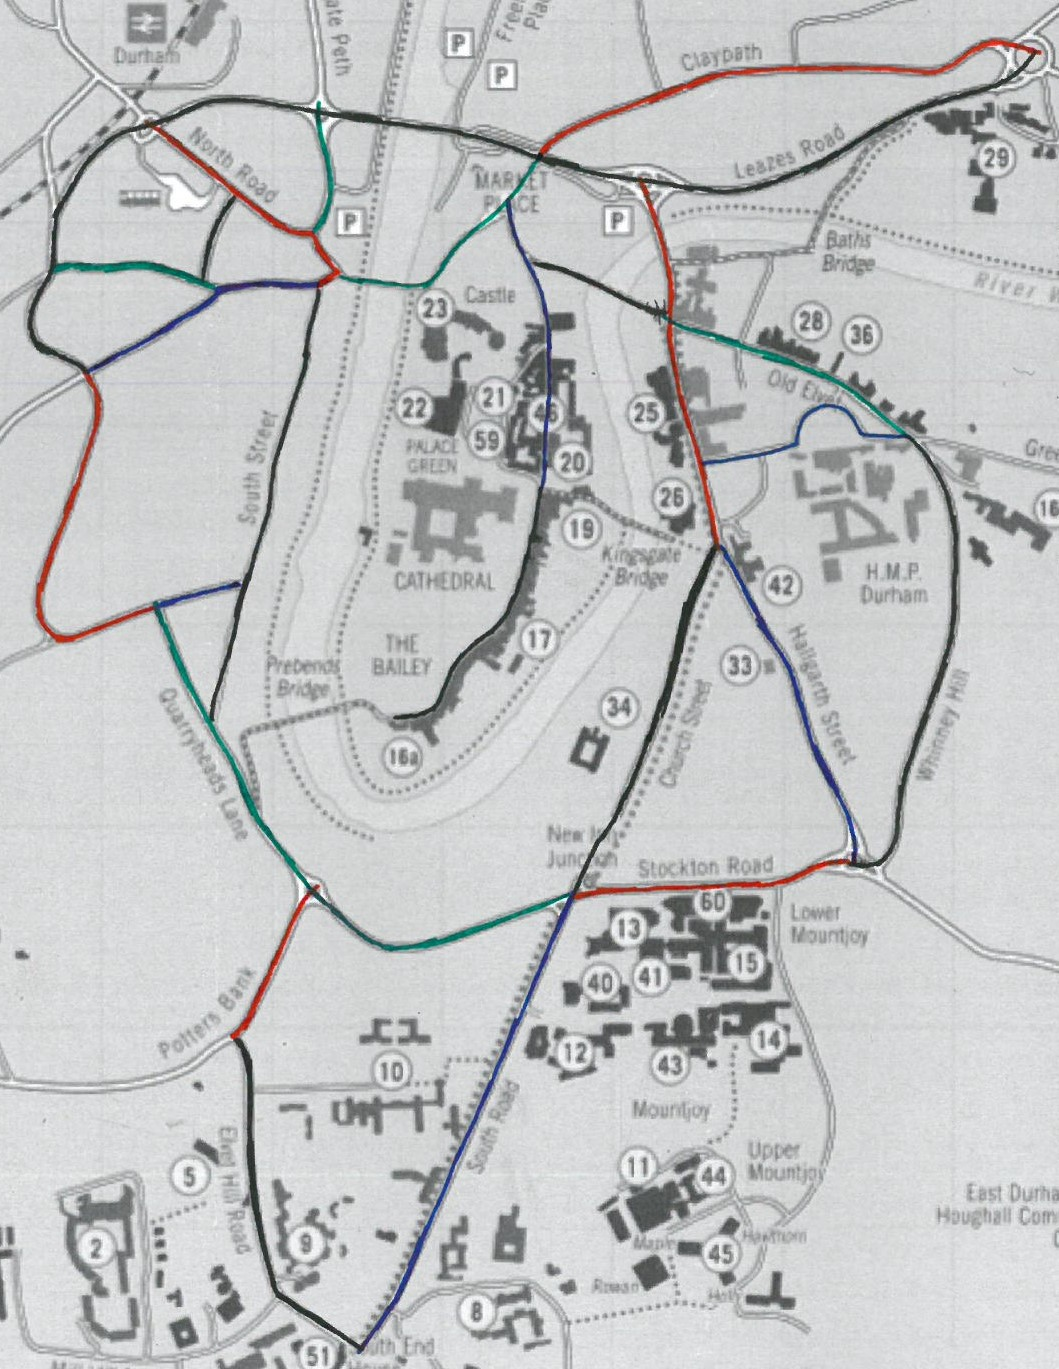
\includegraphics[width=10cm]{durham_with_colour.jpg}
\caption{Durham road network}
\label{durham map}
\end{figure}
\begin{figure}[h]
\centering
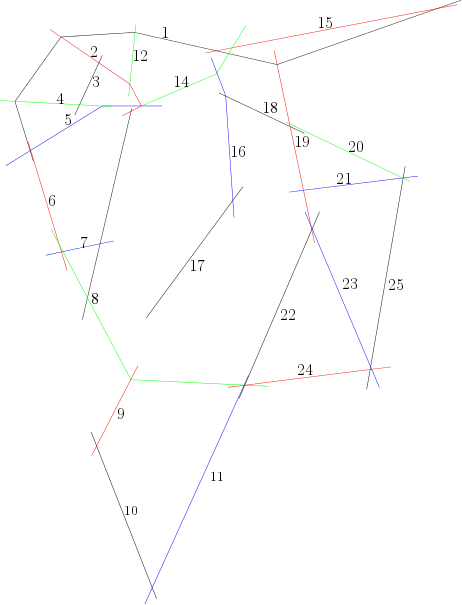
\includegraphics[width=10cm]{axial_colour_label.png}
\caption{Durham road network represented by an axial graph}
\label{durham axial}
\end{figure}

\begin{figure}[h]
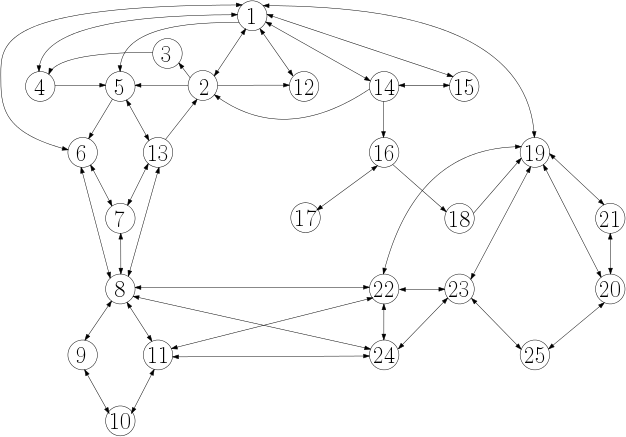
\includegraphics[width=\linewidth]{ipe_durham.png}
\caption{Durham road network represented by a hypergraph}
\label{durham graph}
\end{figure}
\subsubsection{Results and Analysis}
\begin{table}[h] \caption{Comparison of PageRankings produced by standard algorithm and the weighted PageRank algorithm on Durham}
 \centering
 \begin{tabular} {c c| c c} 
 Node & & PR & WPR \\ [0.5ex] 
 \hline
 1&A390&1&1\\
 2&North Rd&8&8\\
 3&Neville St&19&22\\
 4&Allergate&22&19\\
 5&Crossgate&24&24\\
 6&Margery Ln&6&11\\
 7&Grove St&23&23\\
 8&Quarryheads Ln&11&6\\
 9&Potters Bank&13&2\\
 10&Elvet Hill Rd&7&17\\
 11&South Rd&5&18\\
 12&Milburngate&20&25\\
 13&South St&25&13\\
 14&Silver St&2&14\\
 15&Claypath&9&4\\
 16&Saddler St&10&7\\
 17&Bailey&4&5\\
 18&Elvet Bridge&16&20\\
 19&New Elvet&14&5\\
 20&Old Elvet&12&9\\
 21&Court Ln&15&12\\
 22&Church St&21&10\\
 23&Stockton Rd&17&21\\
 24&Hallgarth St&18&16\\
 25&Whinney Hill&3&3\\
 
 \end{tabular}
 \label{Durham comparison}
\end{table}

\subsubsection{Conclusion}

%--------------------Conclusion
\chapter{Conclusion}
%--------------------Bibliography
\addcontentsline{toc}{chapter}{Bibliography}
\bibliographystyle{plain}
\bibliography{bibliography.bib}
%--------------------Appendices

\begin{appendices}
\chapter{Google Matrix}
\begin{align*}
\textbf{G} &  = 0.85\cdot\textbf{H} + (0.85\cdot\textbf{a} + 0.15)\left(\frac{1}{n}\cdot 1^T\right)\\
& = 0.85\cdot\textbf{H} + \left((0.85\left(\begin{array}{c}
0\\0\\0\\0\\0\\0\\1\\0\end{array}\right) + 0.15\left(\begin{array}{c}
1\\1\\1\\1\\1\\1\\1\\1\end{array}\right)\right)\left(\frac{1}{8}\cdot\left(\begin{array}{cccccccc}
1&1&1&1&1&1&1&1\end{array}\right)\right)\\
&= 0.85\left(
\begin{array}{cccccccc}
0 & 0.28\overline{3} & 0 & 0.28\overline{3} & 0 & 0.28\overline{3} & 0 & 0  \\
0 & 0 & 0.425 & 0 & 0.425 & 0 & 0 & 0  \\
0 & 0 & 0 & 0 & 0.850 & 0 & 0 & 0  \\
0 & 0 & 0 & 0 & 0.425 & 0 & 0.425 & 0  \\
0 & 0 & 0 & 0 & 0 & 0 & 0 & 0.850  \\
0 & 0 & 0 & 0.28\overline{3} & 0 & 0 & 0.28\overline{3} & 0.28\overline{3}  \\
0 & 0 & 0 & 0 & 0 & 0 & 0 & 0  \\
0 & 0 & 0 & 0 & 0.425 & 0 & 0.425 & 0  \\
\end{array}
\right) \\&+ \left(
\begin{array}{cccccccc}
0.019 & 0.019 & 0.019 & 0.019 & 0.019 & 0.019 & 0.019 & 0.019  \\
0.019 & 0.019 & 0.019 & 0.019 & 0.019 & 0.019 & 0.019 & 0.019  \\
0.019 & 0.019 & 0.019 & 0.019 & 0.019 & 0.019 & 0.019 & 0.019  \\
0.019 & 0.019 & 0.019 & 0.019 & 0.019 & 0.019 & 0.019 & 0.019  \\
0.019 & 0.019 & 0.019 & 0.019 & 0.019 & 0.019 & 0.019 & 0.019  \\
0.019 & 0.019 & 0.019 & 0.019 & 0.019 & 0.019 & 0.019 & 0.019  \\
0.125 & 0.125 & 0.125 & 0.125 & 0.125 & 0.125 & 0.125 & 0.125  \\
0.019 & 0.019 & 0.019 & 0.019 & 0.019 & 0.019 & 0.019 & 0.019 
\end{array}
\right)\\
&= \left(
\begin{array}{cccccccc}
\frac{3}{160} & \frac{29}{96} & \frac{3}{160} & \frac{29}{96} & \frac{3}{160} & \frac{29}{96} & \frac{3}{160} & \frac{3}{160}  \\
\frac{3}{160} & \frac{3}{160} & \frac{71}{160} & \frac{3}{160} & \frac{71}{160} & \frac{3}{160} & \frac{3}{160} & \frac{3}{160}  \\
\frac{3}{160} & \frac{3}{160} & \frac{3}{160} & \frac{3}{160} & \frac{139}{160} & \frac{3}{160} & \frac{3}{160} & \frac{3}{160}  \\
\frac{3}{160} & \frac{3}{160} & \frac{3}{160} & \frac{3}{160} & \frac{71}{160} & \frac{3}{160} & \frac{71}{160} & \frac{3}{160}  \\
\frac{3}{160} & \frac{3}{160} & \frac{3}{160} & \frac{3}{160} & \frac{3}{160} & \frac{3}{160} & \frac{3}{160} & \frac{139}{160}  \\
\frac{3}{160} & \frac{3}{160} & \frac{3}{160} & \frac{29}{96} & \frac{3}{160} & \frac{3}{160} & \frac{29}{96} & \frac{29}{96}  \\
\frac{1}{8} & \frac{1}{8} & \frac{1}{8} & \frac{1}{8} & \frac{1}{8} & \frac{1}{8} & \frac{1}{8} & \frac{1}{8}  \\
\frac{3}{160} & \frac{3}{160} & \frac{3}{160} & \frac{3}{160} & \frac{71}{160} & \frac{3}{160} & \frac{71}{160} & \frac{3}{160} 
\end{array}
\right) \\
&= \left(
\begin{array}{cccccccc}
0.019 & 0.302 & 0.019 & 0.302 & 0.019 & 0.302 & 0.019 & 0.019  \\
0.019 & 0.019 & 0.444 & 0.019 & 0.444 & 0.019 & 0.019 & 0.019  \\
0.019 & 0.019 & 0.019 & 0.019 & 0.869 & 0.019 & 0.019 & 0.019  \\
0.019 & 0.019 & 0.019 & 0.019 & 0.444 & 0.019 & 0.444 & 0.019  \\
0.019 & 0.019 & 0.019 & 0.019 & 0.019 & 0.019 & 0.019 & 0.869  \\
0.019 & 0.019 & 0.019 & 0.302 & 0.019 & 0.019 & 0.302 & 0.302  \\
0.125 & 0.125 & 0.125 & 0.125 & 0.125 & 0.125 & 0.125 & 0.125  \\
0.019 & 0.019 & 0.019 & 0.019 & 0.444 & 0.019 & 0.444 & 0.019 
\end{array}
\right)
\end{align*}
%--------------------
\chapter{Durham Results}
\begin{figure} [H]  
\begin{equation} \small
\left(
\begin{array}{ccccccccccccccccccccccccc}
0 & \frac{1}{8} & 0 & \frac{1}{8} & \frac{1}{8} & \frac{1}{8} & 0 & 0 & 0  & 0  & 0  & \frac{1}{8} & 0  & \frac{1}{8} & \frac{1}{8} & 0  & 0  & 0  & \frac{1}{8} & 0  & 0  & 0  & 0 & 0  & 0\\
\frac{1}{4} & 0  & \frac{1}{4} & 0  & \frac{1}{4} & 0  & 0  & 0  & 0  & 0  & 0  & \frac{1}{4} & 0  & 0  & 0  & 0  & 0  & 0  & 0  & 0  & 0  & 0  & 0 & 0  & 0 \\
0  & 0  & 0  & 1    & 0  & 0  & 0  & 0  & 0  & 0  & 0  & 0  & 0  & 0  & 0  & 0  & 0  & 0  & 0  & 0  & 0  & 0  & 0 & 0  & 0\\
\frac{1}{2}  & 0  & 0  & 0 & \frac{1}{2}   & 0  & 0  & 0  & 0  & 0  & 0  & 0  & 0  & 0  & 0  & 0  & 0  & 0  & 0  & 0  & 0  & 0  & 0 & 0  & 0\\
0  & 0  & 0  & 0 & 0   & \frac{1}{2} & 0  & 0  & 0  & 0  & 0  & 0  & \frac{1}{2} & 0  & 0  & 0  & 0  & 0  & 0  & 0  & 0  & 0  & 0 & 0  & 0\\
\frac{1}{3} & 0  & 0  & 0 & 0   & 0  & \frac{1}{3} & \frac{1}{3} & 0  & 0  & 0  & 0  & 0  & 0  & 0  & 0  & 0  & 0  & 0  & 0  & 0  & 0  & 0 & 0  & 0\\
0  & 0  & 0  & 0 & 0   & \frac{1}{3} & 0  & \frac{1}{3} & 0  & 0  & 0  & 0  & \frac{1}{3} & 0  & 0  & 0  & 0  & 0  & 0  & 0  & 0  & 0  & 0 & 0  & 0\\
0  & 0  & 0  & 0 & 0   & \frac{1}{7} & \frac{1}{7} & 0  & \frac{1}{7} & 0  & \frac{1}{7} & 0  & \frac{1}{7}  & 0 & 0  & 0  & 0  & 0  & 0  & 0  & 0  & \frac{1}{7} & 0 & \frac{1}{7} & 0\\
0  & 0  & 0  & 0 & 0   & 0  & 0  & \frac{1}{2} & 0  & \frac{1}{2} & 0  & 0  & 0  & 0  & 0  & 0  & 0  & 0  & 0  & 0  & 0  & 0  & 0 & 0  & 0\\
0  & 0  & 0  & 0 & 0   & 0  & 0  & 0  & \frac{1}{2} & 0  & \frac{1}{2} & 0  & 0  & 0  & 0  & 0  & 0  & 0  & 0  & 0  & 0  & 0  & 0 & 0  & 0\\
0  & 0  & 0  & 0 & 0   & 0  & 0  & \frac{1}{4} & 0  & \frac{1}{4} & 0  & 0  & 0  & 0  & 0  & 0  & 0  & 0  & 0  & 0  & 0  & \frac{1}{4} & 0 & \frac{1}{4} & 0\\
1    & 0  & 0  & 0 & 0   & 0  & 0  & 0  & 0  & 0  & 0  & 0  & 0  & 0  & 0  & 0  & 0  & 0  & 0  & 0  & 0  & 0  & 0 & 0  & 0\\
0  & \frac{1}{4} & 0  & 0 & \frac{1}{4}     & 0  & \frac{1}{4}    & \frac{1}{4} & 0  & 0  & 0  & 0  & 0  & 0  & 0  & 0  & 0  & 0  & 0  & 0  & 0  & 0  & 0 & 0  & 0\\
\frac{1}{4} & \frac{1}{4} & 0  & 0 & 0   & 0  & 0  & 0  & 0  & 0  & 0  & 0  & 0  & 0  & \frac{1}{4} & \frac{1}{4} & 0  & 0  & 0  & 0  & 0  & 0  & 0 & 0  & 0\\
\frac{1}{2} & 0  & 0  & 0 & 0   & 0  & 0  & 0  & 0  & 0  & 0  & 0  & 0  & \frac{1}{2} & 0  & 0  & 0  & 0  & 0  & 0  & 0  & 0  & 0 & 0  & 0\\
0  & 0  & 0  & 0 & 0   & 0  & 0  & 0  & 0  & 0  & 0  & 0  & 0  & 0  & 0  & 0  & \frac{1}{2} & \frac{1}{2} & 0  & 0  & 0  & 0  & 0 & 0  & 0\\
0  & 0  & 0  & 0 & 0   & 0  & 0  & 0  & 0  & 0  & 0  & 0  & 0  & 0  & 0  & 1    & 0  & 0  & 0  & 0  & 0  & 0  & 0 & 0  & 0\\
0 & 0  & 0  & 0 & 0   & 0  & 0  & 0  & 0  & 0  & 0  & 0  & 0  & 0  & 0  & 0  & 0  & 0  & 1    & 0  & 0  & 0  & 0 & 0  & 0\\
\frac{1}{4}    & 0  & 0  & 0 & 0   & 0  & 0  & 0  & 0  & 0  & 0  & 0  & 0  & 0  & 0  & 0  & 0  & 0  & 0  & \frac{1}{4} & 0  & \frac{1}{4} & \frac{1}{4}& 0  & 0\\
0  & 0  & 0  & 0 & 0   & 0  & 0  & 0  & 0  & 0  & 0  & 0  & 0  & 0  & 0  & 0  & 0  & 0  & \frac{1}{3} & 0  & \frac{1}{3} & 0  & 0 & 0  & \frac{1}{3}\\
0  & 0  & 0  & 0 & 0   & 0  & 0  & 0  & 0  & 0  & 0  & 0  & 0  & 0  & 0  & 0  & 0  & 0  & \frac{1}{2} & \frac{1}{2} & 0  & 0  & 0 & 0  & 0\\
0  & 0  & 0  & 0 & 0   & 0  & 0  & \frac{1}{5} & 0  & 0  & \frac{1}{5} & 0  & 0  & 0  & 0  & 0  & 0  & 0  & \frac{1}{5} & 0  & 0  & 0  & \frac{1}{5}& \frac{1}{5} & 0\\
0  & 0  & 0  & 0 & 0   & 0  & 0  & 0  & 0  & 0  & 0  & 0  & 0  & 0  & 0  & 0  & 0  & 0  & \frac{1}{4} & 0  & 0  & \frac{1}{4} & 0 & \frac{1}{4} & \frac{1}{4}\\
0  & 0  & 0  & 0 & 0   & 0  & 0  & \frac{1}{5} & 0  & 0  & \frac{1}{5} & 0  & 0  & 0  & 0  & 0  & 0  & 0  & 0  & 0  & 0  & \frac{1}{5} & \frac{1}{5} & 0  & \frac{1}{5}\\
0  & 0  & 0  & 0 & 0   & 0  & 0  & 0  & 0  & 0  & 0  & 0  & 0  & 0  & 0  & 0  & 0  & 0  & 0  & \frac{1}{3} & 0  & 0  & \frac{1}{3} & \frac{1}{3} & 0\\
\end{array}
\right)
\end{equation} 
\caption{Hyperlink matrix for Durham}
\end{figure}  \label{DH}
\begin{figure} [H]  
\begin{equation} \small
\left(
\begin{array}{ccccccccccccccccccccccccc}
0 & \frac{2}{11} & 0 & \frac{1}{11} & \frac{1}{11} & \frac{3}{22} & 0 & 0 & 0  & 0  & 0  & \frac{1}{22} & 0  & \frac{2}{11} & \frac{2}{11} & 0  & 0  & 0  & \frac{2}{11} & 0  & 0  & 0  & 0 & 0  & 0\\
\frac{2}{3} & 0  & \frac{1}{12} & 0  & \frac{1}{6} & 0  & 0  & 0  & 0  & 0  & 0  & \frac{1}{12} & 0  & 0  & 0  & 0  & 0  & 0  & 0  & 0  & 0  & 0  & 0 & 0  & 0 \\
0  & 0  & 0  & 1    & 0  & 0  & 0  & 0  & 0  & 0  & 0  & 0  & 0  & 0  & 0  & 0  & 0  & 0  & 0  & 0  & 0  & 0  & 0 & 0  & 0\\
\frac{4}{5}  & 0  & 0  & 0 & \frac{1}{5}   & 0  & 0  & 0  & 0  & 0  & 0  & 0  & 0  & 0  & 0  & 0  & 0  & 0  & 0  & 0  & 0  & 0  & 0 & 0  & 0\\
0  & 0  & 0  & 0 & 0   & \frac{3}{7} & 0  & 0  & 0  & 0  & 0  & 0  & \frac{4}{7} & 0  & 0  & 0  & 0  & 0  & 0  & 0  & 0  & 0  & 0 & 0  & 0\\
\frac{4}{9} & 0  & 0  & 0 & 0   & 0  & \frac{1}{6} & \frac{7}{18} & 0  & 0  & 0  & 0  & 0  & 0  & 0  & 0  & 0  & 0  & 0  & 0  & 0  & 0  & 0 & 0  & 0\\
0  & 0  & 0  & 0 & 0   & \frac{3}{14} & 0  & \frac{1}{2} & 0  & 0  & 0  & 0  & \frac{2}{7} & 0  & 0  & 0  & 0  & 0  & 0  & 0  & 0  & 0  & 0 & 0  & 0\\
0  & 0  & 0  & 0 & 0   & \frac{3}{26} & \frac{3}{26} & 0  & \frac{1}{13} & 0  & \frac{2}{13} & 0  & \frac{2}{13}  & 0 & 0  & 0  & 0  & 0  & 0  & 0  & 0  & \frac{5}{26} & 0 & \frac{5}{26} & 0\\
0  & 0  & 0  & 0 & 0   & 0  & 0  & \frac{7}{9} & 0  & \frac{2}{9} & 0  & 0  & 0  & 0  & 0  & 0  & 0  & 0  & 0  & 0  & 0  & 0  & 0 & 0  & 0\\
0  & 0  & 0  & 0 & 0   & 0  & 0  & 0  & \frac{1}{3} & 0  & \frac{2}{3} & 0  & 0  & 0  & 0  & 0  & 0  & 0  & 0  & 0  & 0  & 0  & 0 & 0  & 0\\
0  & 0  & 0  & 0 & 0   & 0  & 0  & \frac{7}{19} & 0  & \frac{2}{19} & 0  & 0  & 0  & 0  & 0  & 0  & 0  & 0  & 0  & 0  & 0  & \frac{5}{19} & 0 & \frac{5}{19} & 0\\
1    & 0  & 0  & 0 & 0   & 0  & 0  & 0  & 0  & 0  & 0  & 0  & 0  & 0  & 0  & 0  & 0  & 0  & 0  & 0  & 0  & 0  & 0 & 0  & 0\\
0  & \frac{1}{4} & 0  & 0 & \frac{1}{8} & 0  & \frac{3}{16} & \frac{7}{16} & 0  & 0  & 0  & 0  & 0  & 0  & 0  & 0  & 0  & 0  & 0  & 0  & 0  & 0  & 0 & 0  & 0\\
\frac{1}{2} & \frac{1}{4} & 0  & 0 & 0   & 0  & 0  & 0  & 0  & 0  & 0  & 0  & 0  & 0  & \frac{1}{8} & \frac{1}{8} & 0  & 0  & 0  & 0  & 0  & 0  & 0 & 0  & 0\\
\frac{2}{3} & 0  & 0  & 0 & 0   & 0  & 0  & 0  & 0  & 0  & 0  & 0  & 0  & \frac{1}{3} & 0  & 0  & 0  & 0  & 0  & 0  & 0  & 0  & 0 & 0  & 0\\
0  & 0  & 0  & 0 & 0   & 0  & 0  & 0  & 0  & 0  & 0  & 0  & 0  & 0  & 0  & 0  & \frac{1}{2} & \frac{1}{2} & 0  & 0  & 0  & 0  & 0 & 0  & 0\\
0  & 0  & 0  & 0 & 0   & 0  & 0  & 0  & 0  & 0  & 0  & 0  & 0  & 0  & 0  & 1    & 0  & 0  & 0  & 0  & 0  & 0  & 0 & 0  & 0\\
0 & 0  & 0  & 0 & 0   & 0  & 0  & 0  & 0  & 0  & 0  & 0  & 0  & 0  & 0  & 0  & 0  & 0  & 1    & 0  & 0  & 0  & 0 & 0  & 0\\
\frac{2}{5}    & 0  & 0  & 0 & 0   & 0  & 0  & 0  & 0  & 0  & 0  & 0  & 0  & 0  & 0  & 0  & 0  & 0  & 0  & \frac{3}{20} & 0  & \frac{1}{4} & \frac{1}{5}& 0  & 0\\
0  & 0  & 0  & 0 & 0   & 0  & 0  & 0  & 0  & 0  & 0  & 0  & 0  & 0  & 0  & 0  & 0  & 0  & \frac{4}{9} & 0& \frac{2}{9} & 0  & 0 & 0  & \frac{1}{3}\\
0  & 0  & 0  & 0 & 0   & 0  & 0  & 0  & 0  & 0  & 0  & 0  & 0  & 0  & 0  & 0  & 0  & 0  & \frac{4}{7} & \frac{3}{7} & 0  & 0  & 0 & 0  & 0\\
0  & 0  & 0  & 0 & 0   & 0  & 0  & \frac{7}{22} & 0  & 0  & \frac{2}{11} & 0  & 0  & 0  & 0  & 0  & 0  & 0  & \frac{2}{11} & 0  & 0  & 0  & \frac{2}{11}& 0 & \frac{3}{22}\\
0  & 0  & 0  & 0 & 0   & 0  & 0  & 0  & 0  & 0  & 0  & 0  & 0  & 0  & 0  & 0  & 0  & 0  & \frac{4}{17} & 0  & 0  & \frac{5}{17} & 0 & \frac{5}{17} & \frac{3}{17}\\
0  & 0  & 0  & 0 & 0   & 0  & 0  & \frac{7}{23} & 0  & 0  & \frac{4}{23} & 0  & 0  & 0  & 0  & 0  & 0  & 0  & 0  & 0  & 0  & \frac{5}{23} & \frac{4}{23} & 0  & \frac{3}{23}\\
0  & 0  & 0  & 0 & 0   & 0  & 0  & 0  & 0  & 0  & 0  & 0  & 0  & 0  & 0  & 0  & 0  & 0  & 0  & \frac{1}{4} & 0  & 0  & \frac{1}{3} & \frac{5}{12} & 0\\
\end{array}
\right)
\end{equation} 
\caption{Weighted hyperlink matrix for Durham}
\end{figure}  \label{DWH}
\begin{figure} [H]  
\begin{equation} 
\boldsymbol\pi_{PR} = \left(
\begin{array}{c}
0.0857\\
0.0300\\
0.0124\\
0.0256\\
0.0423\\
0.0557\\
0.0423\\
0.0867\\
0.0289\\
0.0289\\
0.0499\\
0.0215\\
0.0466\\
0.0237\\
0.0201\\
0.0252\\
0.0167\\
0.0167\\
0.0696\\
0.0389\\
0.0107\\
0.0634\\
0.0527\\
0.0601\\
0.0384
\end{array}
\right)    
\boldsymbol\pi_{WPR} = \left(
\begin{array}{c}
0.1023 \\
0.0443 \\
0.0077 \\
0.0313 \\
0.0240 \\
0.0482 \\
0.0295 \\
0.1090 \\
0.0163 \\
0.0126 \\
0.0497 \\
0.0137 \\
0.0379 \\
0.0353 \\
0.0215 \\
0.0093 \\
0.0400 \\
0.0400 \\
0.0691 \\
0.0223 \\
0.0120 \\
0.0785 \\
0.0482 \\
0.0555 \\
0.0396 
\end{array}
\right)
\end{equation} 
\caption{PageRank vector for Durham}
\end{figure}  \label{DPR}

\chapter{Matlab code} \label{app:code}

\begin{lstlisting} [caption=Matlab code for implementing power method taken from \cite{langville} ]
function [pi,time,numiter] = \hbox{PageRank}(pi0,H,n,alpha,epsilon);

% \hbox{PageRank} computes the \hbox{PageRank} vector for an n-by-n Markov
%           matrix H with starting vector pi0 (a row vector)
%           and scaling parameter alpha (scalar). Uses power method.
%
% EXAMPLE: [pi,time,numiter] = \hbox{PageRank}(pi0,H,1000,.9,1e-8)
%
% INPUT: pi0 = starting vector at iteration 0 (row vector)
%        H = row-normalized hyperlink matrix (n-by-n sparse matrix)
%        n = size of H matrix (scalar)
%        alpha = scaling parameter in \hbox{PageRank} model (scalar)
%        epsilon = convergence tolerance (scalar, e.g. 1e-8)
%
% OUTPUT: pi = \hbox{PageRank} vector
%         time = time required to compute \hbox{PageRank} vector
%         numiter = number of iterations until convergence
%        
% Starting vector is usually set to uniform vector,
% pi0=1/n*ones(1,n).
% NOTE: Matlab stores sparse matrices by columns, so it is faster
%       to do some operations on H', the transpose of H.
% get 'a', dangling node vector, where a(i) = 1, if node i 
%    is dangling node and 0 o.w.

rowsumvector = ones(1,n)*H';
nonzerorows=find(rowsumvector);
zerorows=setdiff(1:n,nonzerorows); l=length(zerorows);
a=sparse(zerorows,ones(1,1),ones(1,1),n,1);

k=0;
residual=1;
pi=pi0;
tic;

while(residual>=epsilon)
     prevpi=pi;
     k=k+1;
     pi=alpha*pi*H + (alpha*(pi*a)+1-alpha)*((1/n)*ones(1,n));
     residual=norm(pi-prevpi,1);
end

numiter=k;
time=toc;

\end{lstlisting}

\begin{lstlisting} [caption=Matlab code for implementing HITS power method taken from \cite{langville} ]
function [x,y,time,numiter] = hits[L,x0,n,epsilon]

% HITS computes the HITS authority vector x and hub vector y 
%      for an n-by-n adjacency matrix L with starting vector
%      x0 (a row vector). Uses power method on L'*L.
%
% EXAMPLE: [x,y,time,numiter] = hits[L,x0,100,1e-8]
%
% INPUT: L = adjacency matrix (n-by-n sparse matrix)
%        x0 = starting vector (row vector)
%        n = size of L matrix (integer)
%        epsilon = convergence tolerance (scalar, e.g. 1e-8)
%
% OUTPUT: x = HITS authority vector
%         y = HITS hub vector
%         time = time until convergence
%         numiter = number of iterations until convergence
%        
% The starting vector is usually set to the uniform vector,
% x0=1/n*ones(1/n)

k=0;
residual=1;
x=x0;
tic;

while(residual>=epsilon)
     prevx=x;
     k=k+1;
     x=x*L';
     x=x*L;
     x=x/sum(x);
     residual=norm(x-prevx,1);
end
y=x*L';
y=y/sum(y);
numiter=k;
time=toc;

\end{lstlisting} 
\end{appendices}




\end{document}